\documentclass{beamer}

\usepackage[british]{babel}
\usepackage{graphicx,hyperref,ru,url}
\usepackage{algorithm}
\usepackage{algpseudocode}
\usepackage{subcaption}
\usepackage{ragged2e} 
\usepackage{caption}
\usepackage{tikz}
\usetikzlibrary{shapes,arrows,positioning,fit}
\usepackage{fontawesome}

\def\newblock{\hskip .11em plus .33em minus .07em}
\captionsetup{justification = raggedright, singlelinecheck = false}
\captionsetup[subfigure]{justification=centering,singlelinecheck=false}

%\definecolor{blueone}{RGB}{26,123,242}
%\setbeamercolor{titlelike}{bg=blueone}

\makeatother

\setbeamertemplate{section in toc}
{\leavevmode\leftskip=5ex%
  \llap{%
    \usebeamerfont*{section number projected}%
    \usebeamercolor{section number projected}%
    \begin{pgfpicture}{-1ex}{0ex}{2.7ex}{4ex}
      \color{bg}
      \pgfpathcircle{\pgfpoint{0pt}{.8ex}}{1.9ex}
      \pgfusepath{fill}
      \pgftext[base]{\color{fg}\inserttocsectionnumber}
    \end{pgfpicture}\kern1.25ex%
  }%
  \inserttocsection\par}
\setbeamertemplate{subsection in toc}
  {\leavevmode\leftskip=2em$\bullet$\hskip1em\inserttocsubsection\par}
 
\setbeamertemplate{frametitle continuation}{}  

\title{INTELLIGENT PERSONAL DATA LEAKAGE DETECTION SYSTEM USING DEEP LEARNING AND RULE-BASED ANALYSIS}

\author{\textbf{ABRAR NASSER} \\ \textit{TCR25MCA-2003} \\[0.6cm]     
    Mini Project  \\[13mm]     
    Guided By: \\
    \textbf{Prof. Sankaranrayanan P N} \\[0.3cm]
    Department of Computer Applications
}

\date{}
\setbeamertemplate{caption}[numbered]
\begin{document}

\begin{frame}[plain]
  \titlepage
\end{frame}

\begin{frame}[allowframebreaks]{Outline}
\setlength{\parskip}{1pt}   
\setlength{\itemsep}{2pt}   
\tableofcontents[
    sectionstyle=show/show,     
    subsectionstyle=hide,       
    subsubsectionstyle=hide
]
\end{frame}

\section{Introduction}
\begin{frame}{Introduction}
\begin{itemize}
  \justifying
  \item Rapid growth of digital communication platforms (email, cloud storage, messaging, enterprise systems) has increased the risk of personal data leakage.
  \item Sensitive information such as passwords, financial data, PII, and confidential organizational data is often unintentionally or maliciously exposed.
  \item Rule-based and signature-based systems detect only predefined patterns and lack context awareness.
  \item Conventional machine learning models lack deep contextual understanding of unstructured text.
  \item Encryption and access control mechanisms fail to prevent insider threats once legitimate access has been granted.
\end{itemize}
\end{frame}

\begin{frame}{Introduction - Objectives}
\textbf{Objectives:}
\vspace{0.3cm}
\begin{itemize}
    \justifying
    \item Design an Intelligent Personal Data Leakage Detection System using a unified hybrid pipeline.
    \item Combine rule-based filtering for structured data with Deep Learning (transformer-based NLP) contextual analysis for unstructured text.
    \item Incorporate anomaly-based insider-threat detection to flag irregular behavioral data.
    \item Provide an explainable AI layer so that every detection decision can be understood and acted upon by a security analyst.
\end{itemize}
\end{frame}

\section{System Architecture}
\begin{frame}{System Architecture}
\begin{figure}
\centering
\resizebox{\textwidth}{!}{
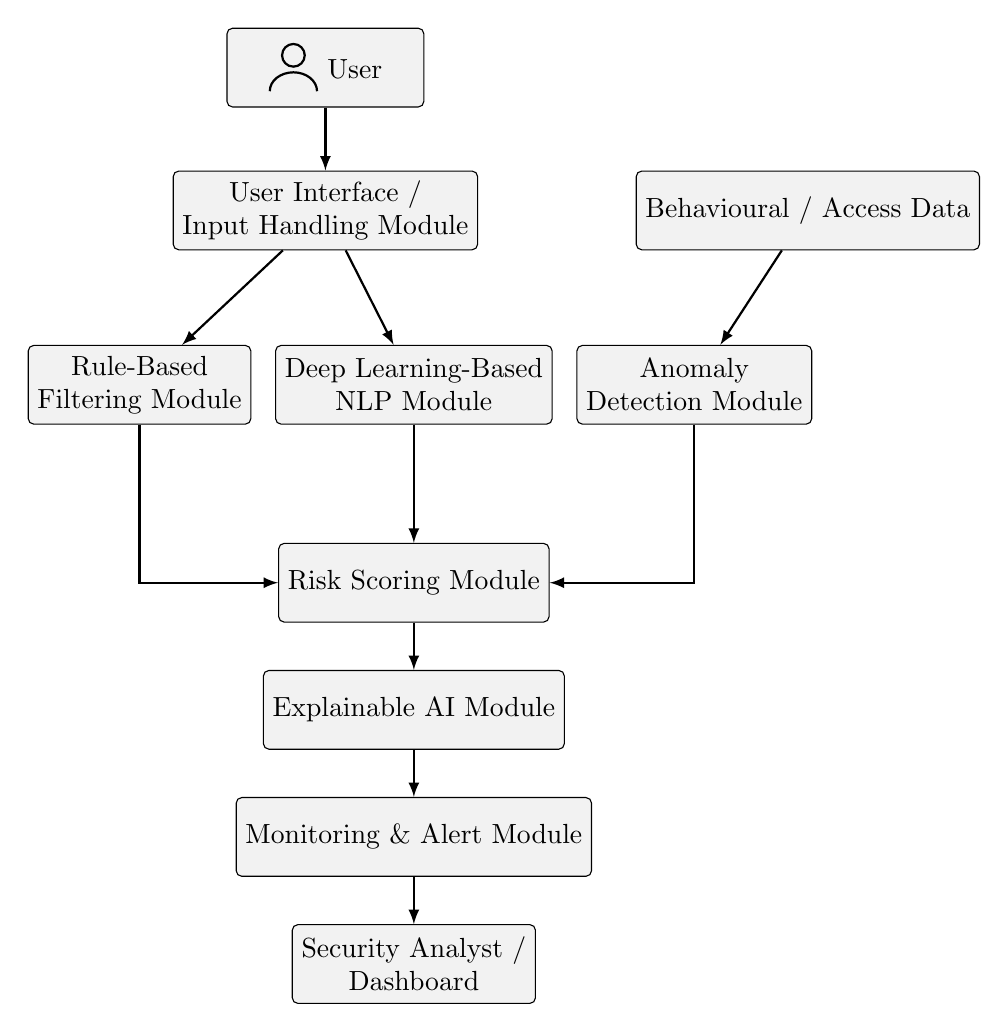
\begin{tikzpicture}[
  node distance=1cm and 0.2cm,
  box/.style={draw, rectangle, align=center, minimum width=2.5cm, minimum height=1cm, fill=gray!10, rounded corners=2pt},
  arrow/.style={-latex, thick}
]
  \newcommand{\outlineuser}{%
    \tikz[baseline=-0.5ex, thick, scale=1.2]{
      \draw (0,0.18) circle (0.12);
      \draw (-0.25,-0.2) arc (180:0:0.25 and 0.2);
    }%
  }
  \node[box] (user) {\outlineuser\ User};
  \node[box, below=0.8cm of user] (ui) {User Interface / \\ Input Handling Module};
  \node[box, right=2cm of ui] (behav) {Behavioural / Access Data};
  
  \node[box, below left=1.2cm and -1cm of ui] (rule) {Rule-Based \\ Filtering Module};
  \node[box, right=0.3cm of rule] (nlp) {Deep Learning-Based \\ NLP Module};
  \node[box, right=0.3cm of nlp] (anomaly) {Anomaly \\ Detection Module};

  \node[box, below=1.5cm of nlp] (risk) {Risk Scoring Module};
  \node[box, below=0.6cm of risk] (xai) {Explainable AI Module};
  \node[box, below=0.6cm of xai] (monitor) {Monitoring \& Alert Module};
  \node[box, below=0.6cm of monitor] (analyst) {Security Analyst / \\ Dashboard};

  \draw[arrow] (user) -- (ui);
  \draw[arrow] (ui) -- (rule);
  \draw[arrow] (ui) -- (nlp);
  \draw[arrow] (behav) -- (anomaly);
  
  \draw[arrow] (rule) |- (risk);
  \draw[arrow] (nlp) -- (risk);
  \draw[arrow] (anomaly) |- (risk);
  
  \draw[arrow] (risk) -- (xai);
  \draw[arrow] (xai) -- (monitor);
  \draw[arrow] (monitor) -- (analyst);
\end{tikzpicture}
}
\caption{System Architecture of the Proposed System}
\end{figure}
\end{frame}

\begin{frame}{System Architecture Description}
\begin{itemize}
  \item The User submits text or documents, which pass through the User Interface Module for validation.
  \item Validated input is analysed in parallel by the Rule-Based Filtering and Deep Learning-Based NLP modules.
  \item The Anomaly Detection Module separately monitors behavioural data for insider-threat indicators.
  \item All outputs converge at the Risk Scoring Module, followed by the Explainable AI Module and the Monitoring \& Alert Module, before reaching the Security Analyst via the dashboard.
\end{itemize}
\end{frame}

\section{Data Flow Diagram}
\begin{frame}{Data Flow Diagrams - Level 0}
\begin{figure}
\centering
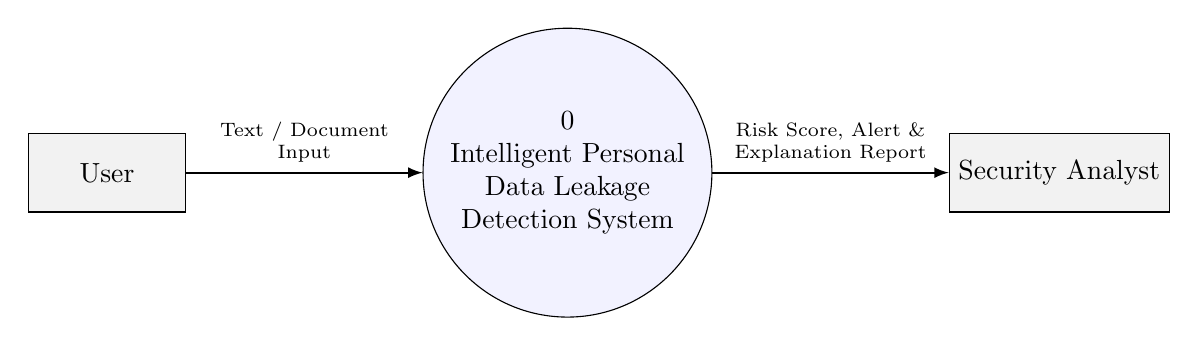
\begin{tikzpicture}[
  node distance=3cm,
  box/.style={draw, rectangle, align=center, minimum width=2cm, minimum height=1cm, fill=gray!10},
  mycircle/.style={draw, circle, align=center, minimum width=3.5cm, fill=blue!5},
  arrow/.style={-latex, thick}
]
  \node[box] (user) {User};
  \node[mycircle, right=of user] (sys) {0 \\ Intelligent Personal \\ Data Leakage \\ Detection System};
  \node[box, right=of sys] (analyst) {Security Analyst};

  \draw[arrow] (user) -- node[above, align=center, font=\scriptsize] {Text / Document \\ Input} (sys);
  \draw[arrow] (sys) -- node[above, align=center, font=\scriptsize] {Risk Score, Alert \& \\ Explanation Report} (analyst);
\end{tikzpicture}
\caption{DFD Level 0}
\end{figure}
\end{frame}

\section{System Implementation}
\begin{frame}[allowframebreaks]{System Implementation}
\begin{itemize}
\justifying
    \item Successfully implemented the core detection pipeline combining Rule-Based Filtering, Deep Learning (NLP), and Anomaly Detection.
    \item \textbf{Backend \& API:} Developed using Python and the Flask framework to handle secure file uploads and API requests.
    \item \textbf{Document Parsing:} Utilizes \texttt{PyPDF2} to automatically extract text and metadata from uploaded PDF documents.
    \item \textbf{Rule-Based Engine:} Employs regular expressions to instantly detect structured PII such as Emails, Phone Numbers, Aadhaar IDs, and Credit Card details.
    \item \textbf{Advanced Detection:} Leverages PyTorch and Hugging Face Transformers (BERT) for deep contextual analysis of unstructured text.
    \item \textbf{Explainability:} Integrated an Explainable AI layer to generate human-readable reports justifying the computed risk scores for the security analyst.
\end{itemize}
\end{frame}

\section{Results and Discussion}
\begin{frame}[allowframebreaks]{Results and Discussion}
\begin{itemize}
\justifying
    \item \textbf{High Accuracy:} The hybrid pipeline combining rule-based regex and deep learning significantly improves precision and reduces false positives compared to standalone methods.
    \item \textbf{Comprehensive Coverage:} Successfully detects both structured PII (emails, IDs) and unstructured, previously unseen sensitive data leakage patterns.
    \item \textbf{Insider Threat Detection:} The behavioral anomaly module efficiently flags irregular data-handling activities, mitigating risks from authorized users.
    \item \textbf{Actionable Insights:} The integrated Risk Scoring combined with Explainable AI (SHAP/LIME) provides transparent, human-readable rationale for every alert, empowering security analysts to act quickly.
    \item \textbf{Performance:} The system operates efficiently, handling both plain text and PDF document parsing with minimal latency, making it suitable for near real-time monitoring.
\end{itemize}
\end{frame}

\begin{frame}{Results - System Dashboard}
    \begin{figure}
        \centering
        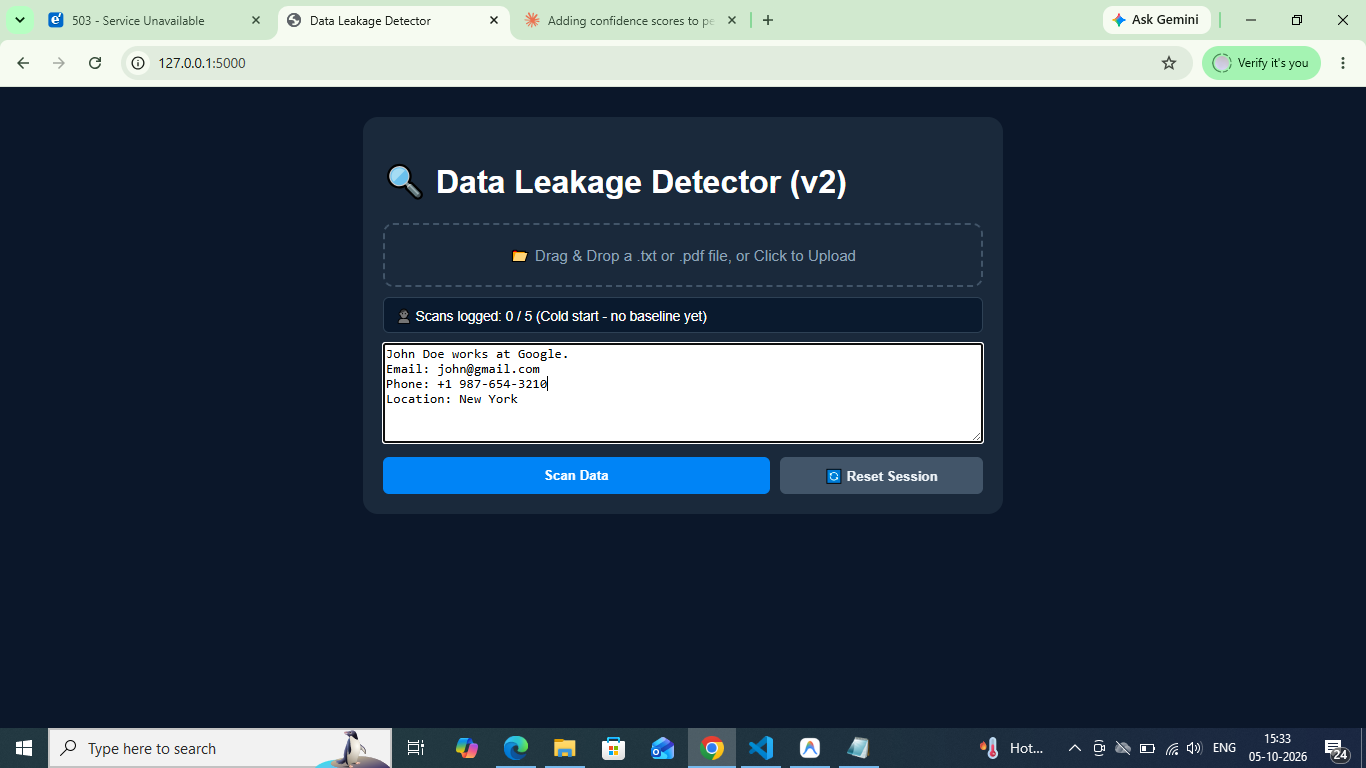
\includegraphics[width=0.9\textwidth,height=0.7\textheight,keepaspectratio]{dashboard.png}
        \caption{System Dashboard Overview}
    \end{figure}
\end{frame}

\begin{frame}{Results - Explainable AI (LIME)}
    \begin{figure}
        \centering
        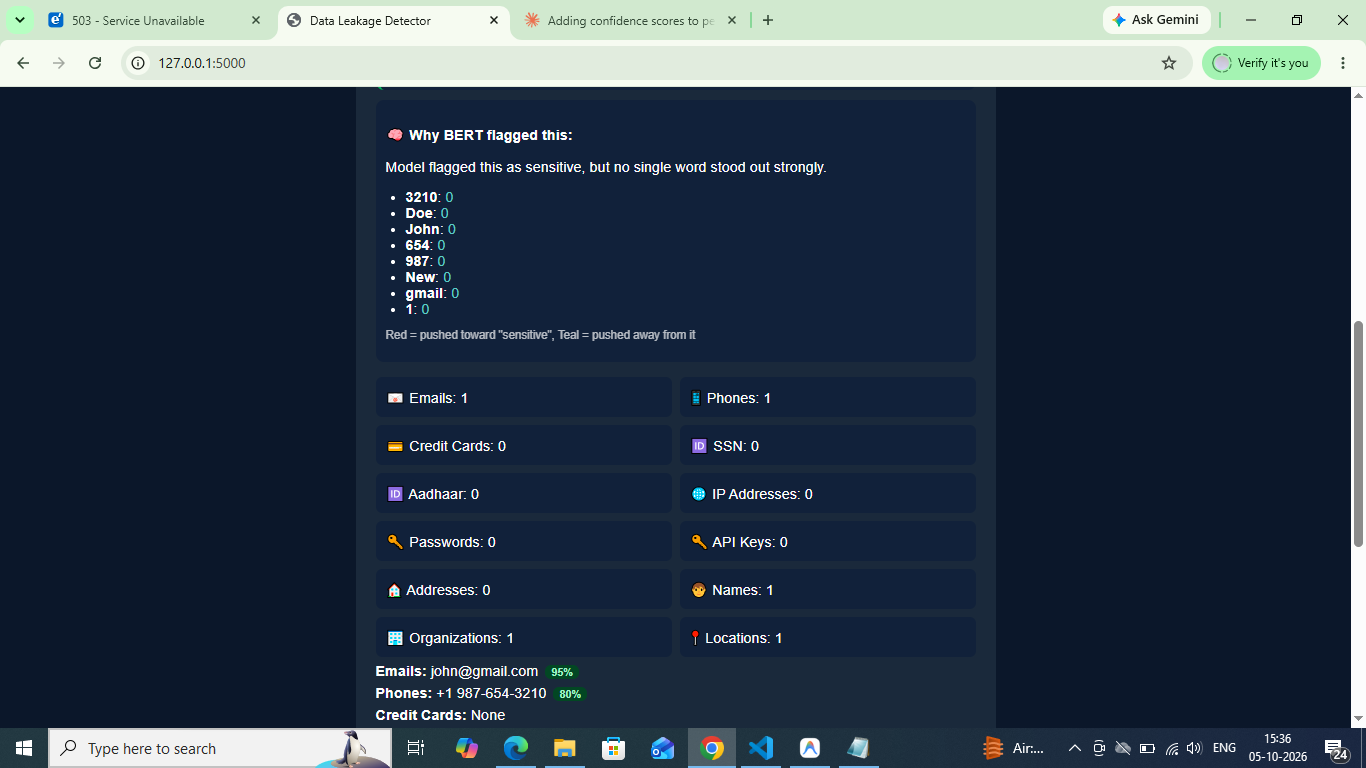
\includegraphics[width=0.9\textwidth,height=0.7\textheight,keepaspectratio]{lime_explaination.png}
        \caption{LIME Explanation for Deep Learning Classification}
    \end{figure}
\end{frame}

\begin{frame}{Results - Anomaly Detection (Normal Baseline)}
    \begin{figure}
        \centering
        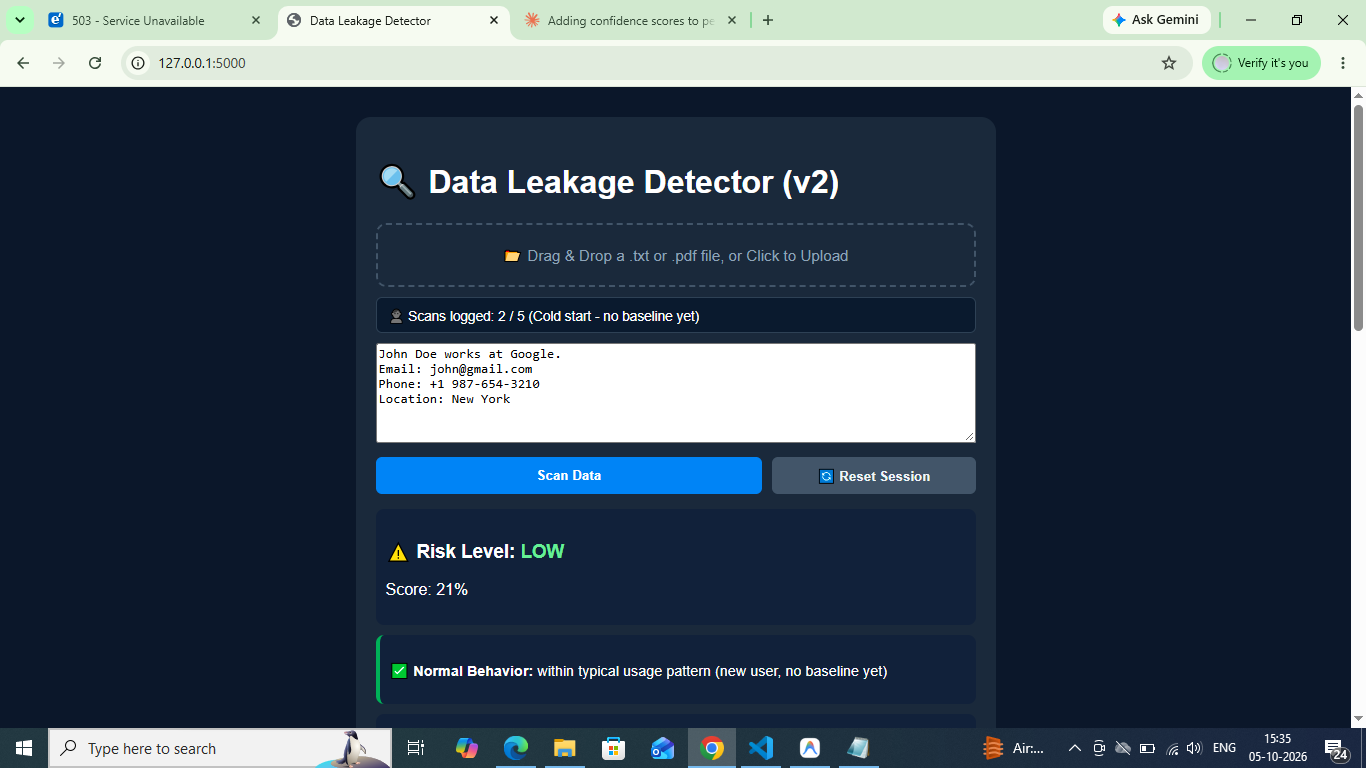
\includegraphics[width=0.9\textwidth,height=0.7\textheight,keepaspectratio]{normal.png}
        \caption{Baseline Normal Behavior Profile}
    \end{figure}
\end{frame}

\begin{frame}{Results - Anomaly Detection (Alert)}
    \begin{figure}
        \centering
        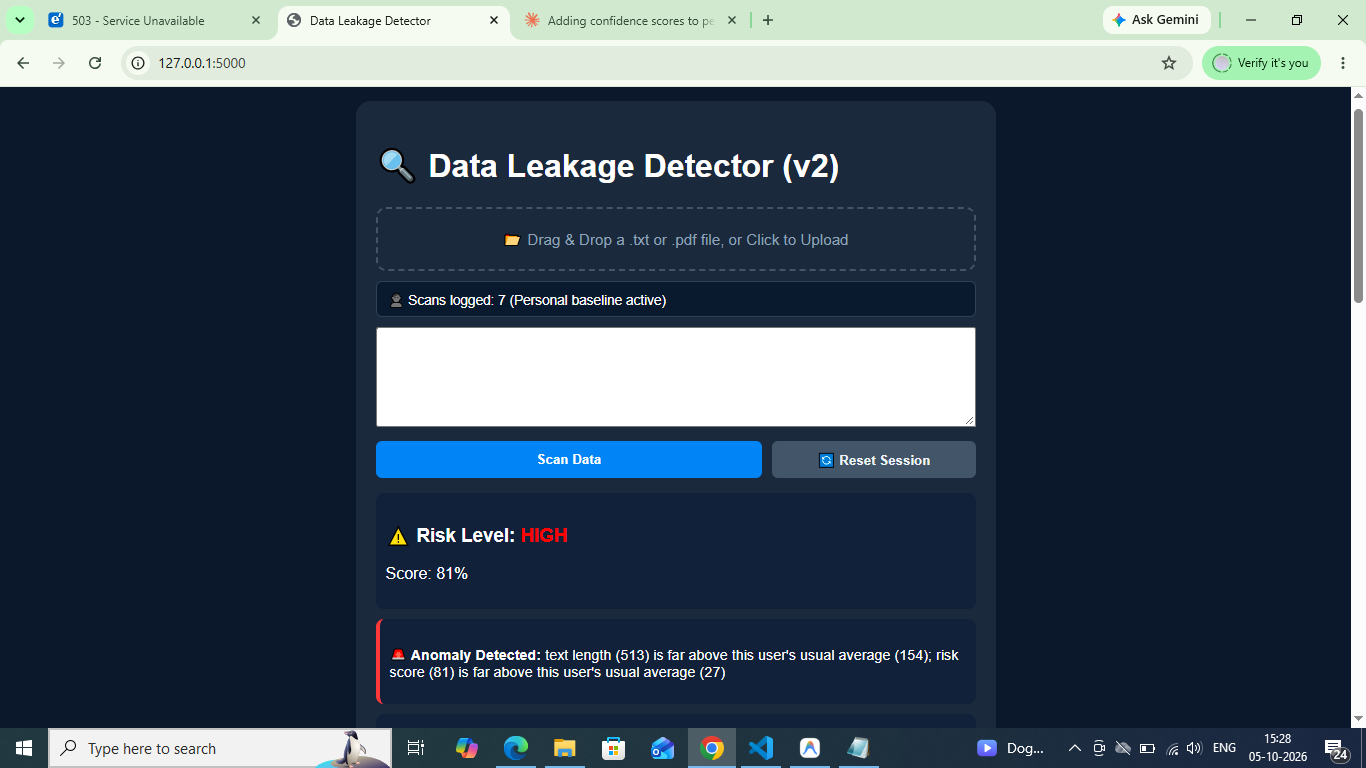
\includegraphics[width=0.9\textwidth,height=0.7\textheight,keepaspectratio]{anomaly.png}
        \caption{Anomaly Detection Alert for Deviant Behavior}
    \end{figure}
\end{frame}

\section{Conclusion}
\begin{frame}{Conclusion}
\begin{itemize}
  \justifying
  \item This project proposes an Intelligent Personal Data Leakage Detection System that unifies rule-based filtering, deep learning (transformer-based NLP) contextual analysis, and behavioural anomaly detection within a single hybrid pipeline.
  \item Combining these complementary techniques allows the system to catch both structured, known leakage patterns and unstructured, previously unseen ones – while an explainable AI layer keeps every decision transparent and actionable for a security analyst.
  \item Overall, the system demonstrates how content-level and behaviour-level signals can be brought together in one pipeline to detect personal data leakage more comprehensively than any single technique used in isolation.
\end{itemize}
\end{frame}

\section{Future Enhancements}
\begin{frame}{Future Enhancements}
\begin{itemize}
\justifying
    \item \textbf{Cloud Integration:} Deploy the detection system on scalable cloud platforms (e.g., AWS, Azure) for enterprise-wide, real-time data monitoring.
    \item \textbf{Expanded File Support:} Extend parsing capabilities beyond PDFs and plain text to include DOCX, Excel, and image-based documents using Optical Character Recognition (OCR).
    \item \textbf{Automated Remediation:} Implement active prevention measures such as auto-redaction of sensitive fields and dynamic blocking of unauthorized data transfers.
    \item \textbf{Advanced Threat Intelligence:} Integrate global threat-intelligence feeds to continuously update and adapt the deep learning models to emerging leakage patterns.
\end{itemize}
\end{frame}

\end{document}
